%% 情報学群実験第3,4(C)用のレポートテンプレート
%
\documentclass[a4j,titlepage]{jarticle}
%% プリアンブルここから
\usepackage[dvipdfmx]{graphicx}
\usepackage{url}
\usepackage{comment}
\usepackage{here}
%
\title{\huge 配達支援システム\\
		外部設計書}
\author{第2.0版\\
        ONO-Systems\\}
\date{\today}

%本文
\begin{document}
\maketitle

%目次
\tableofcontents
\clearpage

\section{目的}
現在,日本で行われている形態の宅配便サービスが開始し,約40年ほど経過しています.近年のECサイトの拡大に伴い,食料品や日用雑貨などを購入する利用者も増えており,ネットショッピングは特別な商品を買う場所ではなく,近所への買い物と似たような感覚で利用する人々が増えているため,宅配便の取扱個数はさらなる増加が予想されます\cite{ref1}.\\
\ \ \ その一方で,全体の取扱個数の中でも約2割ほどが再配達になっており,さらに約4割の利用者が「配達されることを知らなかった」という調査結果が国土交通省の調査により明らかになっています(図2).この2割にのぼる再配達を労働力に単純に換算すると年間約9万人もの労働力に相当するとも言われています.また,再配達によりトラックなどから排出される二酸化炭素によって,地球温暖化問題にも影響を与えています.さらに,再配達と宅配便の取扱個数の増加により,配達員の長時間労働などの問題が生じ,配達員の人手不足も深刻になっています\cite{ref1}.\\
\ \ \ 利用者側からすると商品が届いて不在票をもらう前に,利用者側から容易に配達員に受け取りの可否を連絡することは難しいです.\\
%=====================================
\ \ \ そこで,弊社では情報技術を駆使することにより宅配業務における配達員の負担を軽減し,消費者の利便性にも配慮した配達支援システムを提案します.
%=====================================

\section{用語の定義}
本システムでは以下のように用語を定義します.
\begin{itemize}
 \item 利用者:ネットショッピングなどを通じて商品を購入して,自宅に配送するように指定した消費者
 \item 配達員:宅配業者の従業員で商品をお客様の家まで届ける人
 \item ユーザ:本システムを利用する利用者と配達員を合わせたもの
 \item マーカー:荷物の一覧表示時に荷物情報の左側に表示される円形のもの
 \item ピン:マップ表示時に利用者の住所を示す涙滴型のもの
 \item 現在地マーカー:マップ表示画面で配達員の現在地を示すもの
\end{itemize}

\section{システム概要}
ここでは,システムの機能概要を説明します.本システムは荷物を受け取れるか否を一般利用者に選択させ,配達員に不要な荷物を運ばせないことで宅配業者の負担を軽減し,荷物配達を支援するシステムです.

\subsection{サブシステムの概要}
本システム内を構築するためのサブシステムの概要を以下に示します.本システムはのサブシステムは利用者側,配達員側,管理者側の3つに大別されます.

\subsection{サブシステム(利用者)}
本システム内を構築するためのサブシステムの概要を以下に示します.

\subsubsection{荷物情報一覧表示サブシステム}
利用者側または配達員側の荷物情報を一覧で表示させます.利用者側は時間順,配達員側は距離順+時間順で表示されます.受け取り可否情報が"可"であれば緑色のマーカー,"否"であれば赤色のマーカー,"未選択"であれば灰色のマーカーが表示されます.利用者側,配達員側ともに指定された条件による絞込みが可能です.\\
『荷物情報表示機能』,『荷物情報絞込み機能』によって構成されています.
\begin{itemize}
\item \textbf{荷物情報表示機能} \\
入力: なし \\
出力: 荷物情報データ(受け取り可否情報,配達元,商品名,伝票番号,配達先,配達希望時間帯)  \\
処理: 荷物情報データを読み出し,枠内に表示します.
\item \textbf{荷物情報絞込み機能} \\
入力: なし \\
出力: 絞込み条件に合致した荷物情報 \\
処理: 荷物情報データを読み出し,各条件に従い表示するか否かを判断します.
\end{itemize}

\subsubsection{荷物情報詳細表示サブシステム}
利用者が持つ荷物の内,ひとつの荷物に対しての情報すべてを表示し,荷物情報の詳細を確認することができます.\\
『荷物情報詳細表示機能』によって構成されています.
\begin{itemize}
\item \textbf{荷物情報詳細表示機能} \\
入力: なし \\
出力: 荷物情報データ(ALL) \\
処理: 荷物情報データを読み出しすべて表示します.
\end{itemize}

\subsubsection{配達物受け取り可否選択サブシステム}
位置情報通知サブシステムによって表示された通知または荷物詳細情報から配達物の受け取り可否を選択できます.受け取り可否が利用者によって選択されるとその結果をデータベースに送信します.\\
『受け取り可否送信機能』によって構成されています.
\begin{itemize}
\item \textbf{受け取り可否送信機能} \\
入力: 選択結果(可,否) \\
出力: なし \\
処理: 利用者が選択した受け取り可否の結果をデータベースに登録します.
\end{itemize}

\subsubsection{配達日時選択サブシステム}
荷物詳細情報から配達物の配達日時を変更できます.配達日時が利用者によって選択されるとその結果をデータベースに送信します.\\
『配達日時変更機能』によって構成されています.
\begin{itemize}
\item \textbf{配達日時送信機能} \\
入力: 配達日時選択結果\\
出力: なし \\
処理: 利用者が選択した配達日時をデータベースに登録します.
\end{itemize}

\subsubsection{アカウント操作サブシステム}
名前,メールアドレス,パスワード,パスワードの再入力,電話番号をアカウント情報としてアカウントを登録します.また,ログイン画面にてメールアドレスとパスワードを入力することで,登録したアカウントにログインできます.ログインをしなければ全てのサブシステムを利用できません.またパスワードを忘れた場合はアカウント作成の際に登録したメールアドレス宛にパスワード再発行の為のメールを送信します. \\
『アカウント作成機能』,『パスワード再設定機能』,『ログイン機能』によって構成されています.
\begin{itemize}
\item \textbf{アカウント作成機能} \\
入力: ユーザデータ(名前,メールアドレス,パスワード,電話番号) \\
出力: なし \\
処理: 入力されたユーザデータをデータベースへ登録します.
\item \textbf{パスワード再設定機能} \\
入力: ユーザデータ(メールアドレス) \\
出力: メール \\
処理: 入力されたメールアドレスに対しパスワード再設定用の画面に遷移出来るURLを含む電子メールを送信します.その後新しいパスワードをデータベースに送信します.
\item \textbf{ログイン機能} \\
入力: ユーザデータ(ID,パスワード) \\
出力: ログイン \\
処理: 入力されたIDとパスワードからアカウントを特定しログインを行います.
\end{itemize}

\newpage

\subsection{サブシステム(配達員)}
本システム内を構築するためのサブシステムを以下に示します.

\subsubsection{荷物情報一覧表示サブシステム}
利用者側または配達員側の荷物情報を一覧で表示させます.利用者側は時間順,配達員側は距離順+時間順で表示されます.受け取り可否情報が"可"であれば緑色のマーカー,"否"であれば赤色のマーカー,"未選択"であれば灰色のマーカーが表示されます.利用者側,配達員側ともに指定された条件による絞込みが可能です.\\
『荷物情報表示機能』,『荷物情報絞込み機能』によって構成されています.
\begin{itemize}
\item \textbf{荷物情報表示機能} \\
入力: なし \\
出力: 荷物情報データ(受け取り可否情報,配達元,商品名,伝票番号,配達先,配達希望時間帯)  \\
処理: 荷物情報データを読み出し,枠内に表示します.
\item \textbf{荷物情報絞込み機能} \\
入力: なし \\
出力: 絞込み条件に合致した荷物情報 \\
処理: 荷物情報データを読み出し,各条件に従い表示するか否かを判断します.
\end{itemize}

\subsubsection{荷物情報詳細表示サブシステム}
配達員が持つ荷物の内,ひとつの荷物に対しての情報すべてを表示し,荷物情報の詳細を確認することができます.\\
『荷物情報詳細表示機能』によって構成されています.
\begin{itemize}
\item \textbf{荷物情報詳細表示機能} \\
入力: なし \\
出力: 荷物情報データ(ALL) \\
処理: 荷物情報データを読み出しすべて表示します.
\end{itemize}


\subsubsection{配達日時選択サブシステム}
荷物詳細情報から配達物の配達日時を変更できます.配達日時が配達員によって選択されるとその結果をデータベースに送信します.\\
『配達日時変更機能』によって構成されています.
\begin{itemize}
\item \textbf{配達日時送信機能} \\
入力: 配達日時選択結果\\
出力: なし \\
処理: 配達員が選択した配達日時をデータベースに登録します.
\end{itemize}

\subsubsection{配達完了選択サブシステム}
配達員は荷物詳細情報から配達物の配達完了または配達未完了を選択することがでます.配達完了が配達員によって選択されるとその結果をデータベースに送信します.\\
『配達完了フラグ送信機能』によって構成されています.
\begin{itemize}
\item \textbf{配達完了フラグ送信機能} \\
入力: 配達完了選択結果\\
出力: なし \\
処理: 配達員が選択した結果をデータベースに登録します.
\end{itemize}

\subsubsection{位置情報通知サブシステム}
配達員が利用者の住所に近づいた場合またはトラックに荷物を運びこむ営業所の時点で,配達員の位置情報を受信できます.配達員の位置情報データと利用者の住所データの差分から距離を算出し,一定以下になった場合に利用者側アプリケーションに荷物受け取りの可否を問う旨の通知を表示します.\\
『位置情報取得機能』,『距離算出機能』,『通知表示機能』によって構成されています。
\begin{itemize}
\item \textbf{位置情報取得機能} \\
入力: 位置情報データ(緯度,経度) \\
出力: なし \\
処理: 一定時間毎に配達員の位置情報データを取得し,データベースに保存します.
\item \textbf{距離算出機能} \\
入力: 利用者の住所データ(緯度,経度),位置情報データ(緯度,経度) \\
出力: なし \\
処理: Google Maps APIを用いて,配達員の位置情報データの緯度経度と利用者の住所データの緯度経度から2点間の距離を算出し,保存します.
\item \textbf{通知表示機能} \\
入力: 2点間の距離 \\
出力: 受け取りの可否を問う通知 \\
処理: 2点間の距離が一定以下になった場合に利用者側アプリケーションに通知を表示します.
\end{itemize}

\subsubsection{音声読み上げサブシステム}
配達物の受け取り可否選択サブシステムによって荷物情報データが更新された場合に配達員側アプリケーション上で利用者の選択した受け取り可否の結果を合成音声によって読み上げます. \\
『音声読み上げ機能』によって構成されています.
\begin{itemize}
\item \textbf{音声読み上げ機能} \\
入力: 荷物情報データ(利用者名,選択結果(可/否)) \\
出力: 合成音声\\
処理: 音声合成APIを用いて音声を合成し,利用者名及び更新された選択結果を読み上げます.
\end{itemize}

%\subsubsection{配達物の受け取り可否選択サブシステム}
%利用者は配達物の受け取り可否を選択することができ,その選択結果は配達員に送信されます.

\subsubsection{受け取り可否の地図上表示サブシステム}
荷物情報データを読み出し,その受け取り可否情報や利用者データをマップ上にピン及びテキストとして表示します.受け取り可否情報によってマップ上に表示されるピンの色が変わり,受け取り可否情報が"可"であれば緑色のピン,"否"であれば赤色のピン,"未選択"であれば灰色のピンが表示されます.テキスト部分には利用者名,住所,配達希望時間帯が表示されます. \\
『現在地情報表示機能』,『受け取り可否表示機能』,『荷物情報表示機能』,『荷物情報絞込み機能』によって構成されています.
\begin{itemize}
\item \textbf{現在地情報表示機能} \\
入力: 位置情報 \\
出力: 現在地マーカー \\
処理: 配達員端末のGPS機能を用いて配達員の位置情報を取得し,その位置を現在地マーカーとして表示します.
\item \textbf{受け取り可否表示機能} \\
入力: 選択結果(可/否) \\
出力: ピン \\
処理: Google Maps APIを用いて受け取り可否情報をマップ上にピンとして表示します.
\item \textbf{荷物情報表示機能} \\
入力: なし \\
出力: 荷物情報データ(利用者名,住所,配達希望時間帯) \\
処理: 利用者名,住所,配達希望時間帯を枠に囲まれたテキストとして表示します.
\item \textbf{荷物情報絞込み機能} \\
入力: 絞込み選択結果 \\
出力: ピンおよび荷物情報 \\
処理: 荷物情報データを読み出し,各条件に従い表示するか否かを判断します.
\end{itemize}

\subsubsection{アカウント操作サブシステム}
ログイン画面にてメールアドレスとパスワードを入力することで,あらかじめ管理者より配布されたアカウントにログインできます.ログインをしなければ全てのサブシステムを利用できません.またパスワードを忘れた場合は指定されたメールアドレス宛にパスワード再発行の為のメールを送信します. \\
『パスワード再設定機能』,『ログイン機能』によって構成されています.
\begin{itemize}
\item \textbf{パスワード再設定機能} \\
入力: ユーザデータ(メールアドレス) \\
出力: メール\\
処理: 入力されたメールアドレスに対しパスワード再設定用の画面に遷移出来るURLを含む電子メールを送信します.その後新しいパスワードをデータベースに送信します.
\item \textbf{ログイン機能} \\
入力: ユーザデータ(ID,パスワード) \\
出力: ログイン \\
処理: 入力されたIDとパスワードからアカウントを特定しログインを行います.
\end{itemize}


\subsection{サブシステム(管理者)}
本システム内を構築するためのサブシステムの概要を以下に示します.

\subsubsection{アカウント管理サブシステム}
管理者はユーザアカウントの閲覧,作成,編集,削除ができます.これらの機能により管理者は配達員アカウントを一度に複数作成でき,営業所の配達員全員にアカウントを付与するという操作などが可能です\\
『ユーザアカウント閲覧機能』,『ユーザアカウント管理機能』によって構成されています.
\begin{itemize}
\item \textbf{ユーザアカウント閲覧機能} \\
入力: なし \\
出力: ユーザアカウントデータ(ALL) \\
処理: 現在存在するユーザアカウントをテーブル形式のテキストで表示します.
\item \textbf{ユーザアカウント管理機能} \\
入力: 操作結果(作成,編集,削除) \\
出力: なし \\
処理: ユーザアカウントの操作(作成,編集,削除)をデータベースに送信し登録します.
\end{itemize}

\newpage

\section{利用者インタフェース設計書}
ここでは,利用者が用いる際に使用する利用者インターフェースの設計を示します.

\subsection{画面遷移図}

\begin{figure}[H]
 \begin{center}
  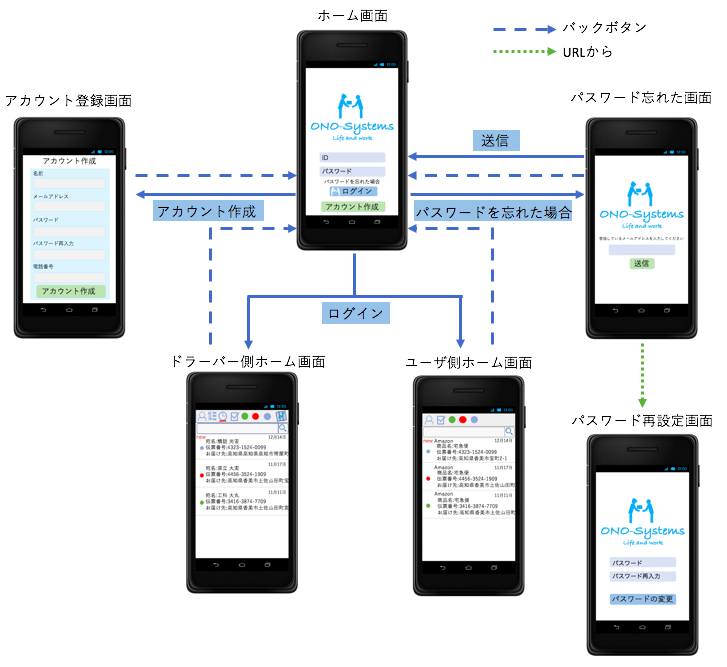
\includegraphics[width=150mm]{screen_transition_home.png}
	\caption{画面遷移図ホーム画面}
	\label{fig:screen_transition_home}
 \end{center}

\end{figure}

\begin{figure}[H]
 \begin{center}
  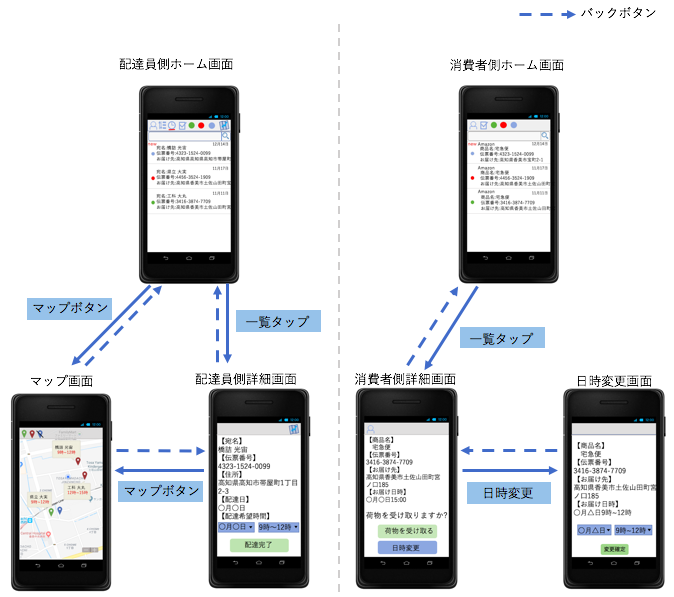
\includegraphics[width=130mm]{screen_transition_login.png}
	\caption{画面遷移図ログイン画面}
	\label{fig:screen_transition_login}
 \end{center}

\end{figure}

\begin{figure}[H]
 \begin{center}
  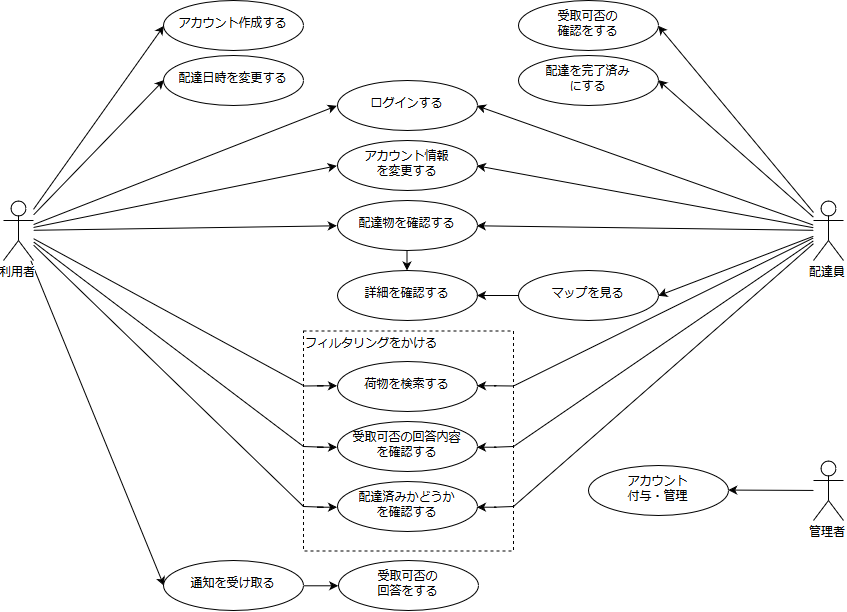
\includegraphics[width=150mm]{use_case.png}
	\caption{ユースケース図}
	\label{fig:use_case}
 \end{center}

\end{figure}

\newpage
\subsection{共有画面詳細}
ここでは配達支援システムの共有画面詳細について記します.

\subsubsection{ホーム画面}
図\ref{fig:login}は配達支援システムのホーム画面です.この画面はログインしていない状態でアプリを起動した時に表示されるます.また,この画面から「ログイン」,「アカウント作成」,「パスワードを忘れた場合」に遷移します.

\begin{figure}[H]
 \begin{center}
  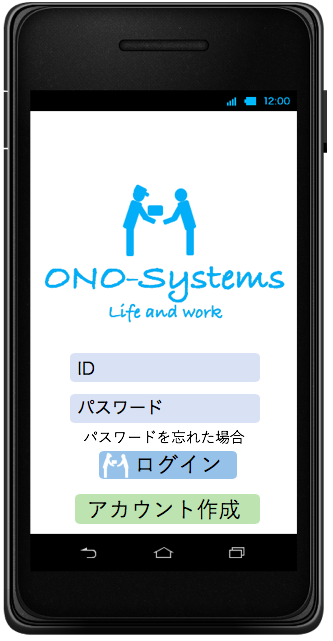
\includegraphics[width=100mm]{login.png}
	\caption{ログイン画面}
	\label{fig:login}
 \end{center}

\end{figure}

\newpage
\subsubsection{パスワードを忘れた場合の画面}
図\ref{fig:ps_lost}は配達支援システムのパスワードを忘れた場合の画面です.この画面はホーム画面の「パスワードを忘れた場合」をタップすると表示されます.画面中央部の枠に既に登録してあるメールアドレスを入力し,送信をタップするとそのメールアドレスにパスワード再発行の為のURLが送られます.

\begin{figure}[H]
 \begin{center}
  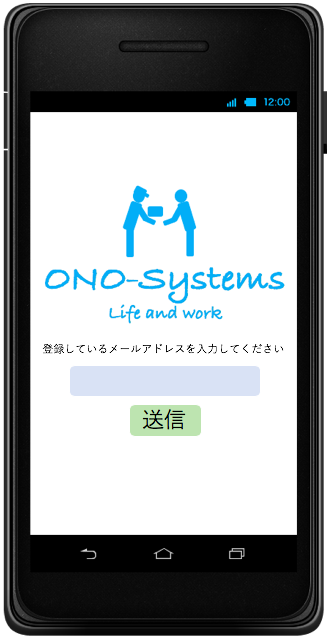
\includegraphics[width=50mm]{ps_lost.png}
	\caption{パスワードを忘れた場合の画面}
	\label{fig:ps_lost}
 \end{center}

\end{figure}
\newpage
\subsubsection{パスワード再設定画面}
図\ref{fig:ps_change}は配達支援システムのパスワード再設定画面です.この画面は再発行の為のURLをタップすると表示されます.画面中央部の枠にパスワードを二回入力し,「パスワードの変更」をタップするとパスワード再発行が完了します.

\begin{figure}[H]
 \begin{center}
  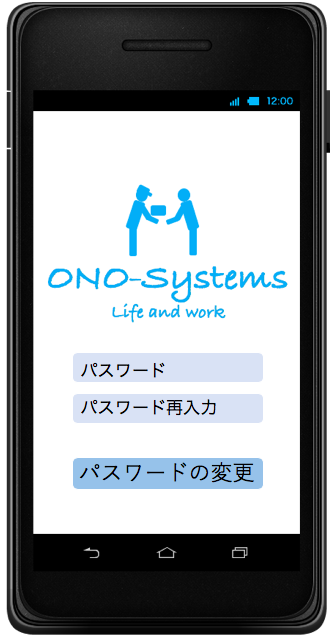
\includegraphics[width=50mm]{ps_change.png}
	\caption{パスワード再設定画面}
	\label{fig:ps_change}
 \end{center}

\end{figure}
\newpage
\subsubsection{アカウント作成画面}
図\ref{fig:account_create}は配達支援システムのアカウント作成画面です.この画面はホーム画面の「アカウント作成」をタップすると表示されます.画面の入力欄に名前,メールアドレス,パスワード,パスワードの再入力,電話番号を入力し,「アカウント作成」をタップするとアカウントを作成することができます.アカウント作成後は利用者ホーム画面に遷移します.

\begin{figure}[H]
 \begin{center}
  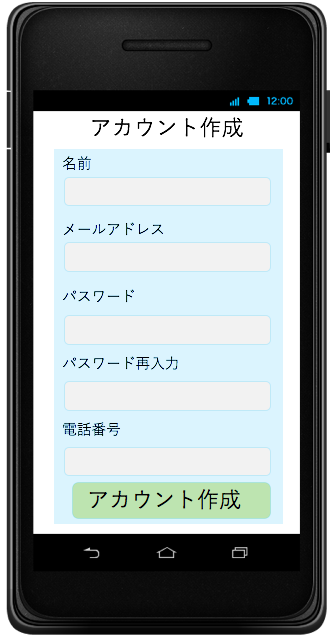
\includegraphics[width=50mm]{account_create.png}
	\caption{アカウント作成画面}
	\label{fig:account_create}
 \end{center}

\end{figure}

\subsection{配達員側画面詳細}
ここでは配達支援システムの配達員側画面詳細について記します.

\subsubsection{ホーム画面}
図\ref{fig:driver_home}は配達支援システムの配達員のホーム画面です.この画面はログイン画面でID,パスワードを入力し,ログインした場合に表示されます.また,既にログインしている場合はアプリ起動時に表示されます.この画面の機能は下記にて説明します.
\begin{enumerate}
	\item 利用者の選択結果のリアルタイム表示機能\\
	 \ 利用者の荷物受け取りの可否をリアルタイムに画面表示します.配達員が未読の間は各欄の左側に「new」と表示されます.
	\item 利用者情報ボタン\\
	 \ 利用者のアカウント情報を表示,編集するサイドバーを出すことができます.
	\item 距離順ソートボタン\\
	 \ 配達員から配達先までの距離を近い順にソートします.
	\item 時間順ソートボタン\\
   \ 時間指定の期限が短い順にソートします.
	\item 配達済みソートボタン\\
   \ 配達完了状態の荷物の表示・非表示を選択できます.
	\item 受け取り可否別表示ボタン\\
	 \ 「受け取れる」,「受け取れない」,「未選択」の三つを好きに表示・非表示できます.
	\item マップボタン\\
   \ マップ画面に遷移します.
	\item 検索バー\\
	 \ 入力された文字と一致する荷物を配達時間順(+距離?)に表示します.
\end{enumerate}

\begin{figure}[H]
 \begin{center}
  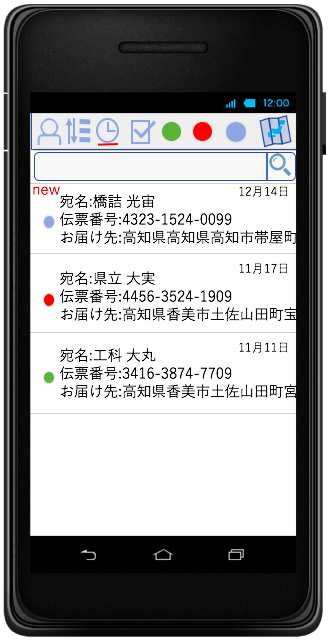
\includegraphics[width=100mm]{driver_home.png}
	\caption{ホーム画面}
	\label{fig:driver_home}
 \end{center}

\end{figure}



\newpage
\subsubsection{サイドバー画面}
図\ref{fig:driver_side}は配達支援システムのサイドバーの画面です.この画面はホーム画面の「利用者情報ボタン」をタップすると表示されます.画面の各欄には利用者の情報(名前,メールアドレス,パスワード,パスワード再入力,電話番号)が表示されており,変更したい部分を書き換えた後に更新ボタンを押すことで利用者情報を変更することができます.また,画面中央上部の「×」ボタンまたはバックボタンをタップするとホーム画面に遷移します.

\begin{figure}[H]
 \begin{center}
  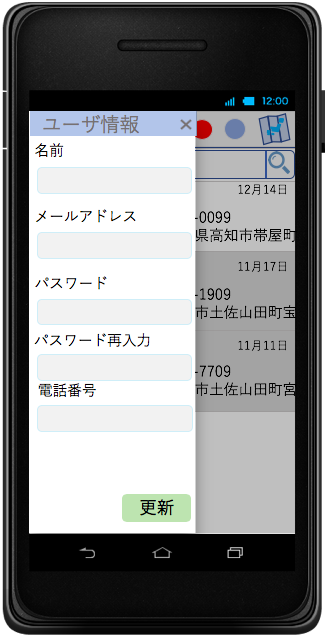
\includegraphics[width=50mm]{driver_side.png}
	\caption{サイド画面}
	\label{fig:driver_side}
 \end{center}

\end{figure}
\newpage
\subsubsection{詳細画面}
図\ref{fig:driver_details}は配達支援システムの詳細画面です.この画面はホーム画面の各荷物欄をタップすると表示されます.画面には配達先の情報(宛名,伝票番号,住所,配達希望時間)が表示されており,プルダウン,更新ボタン,配達完了ボタン,マップボタンがあります.プルダウンでは配達希望時間を選ぶことができ,配達希望時間を変更した後に更新ボタンをタップすると配達希望時間を変更することができます.また,画面下の配達完了ボタンをタップすると配達完了状態にでき,画面右上のマップボタンをタップするとマップ画面へ遷移することができます.
\begin{figure}[H]
 \begin{center}
  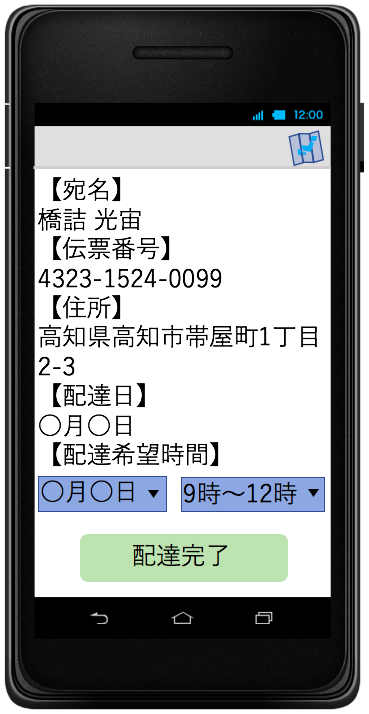
\includegraphics[width=50mm]{driver_details.png}
	\caption{詳細画面}
	\label{fig:driver_details}
 \end{center}

\end{figure}



\newpage
\subsubsection{マップ画面}
図\ref{fig:map}は配達支援システムのマップ画面です.この画面はホーム画面,配達員詳細画面のマップボタンをタップすると表示されます.この画面の機能は下記で説明します.
\begin{enumerate}
	\item 配達先表示機能\\
	 \ 各ピンの場所に住所と配達指定時間が表示されます.下記で説明する絞り込み機能を使用している色は非表示になります.
	\item 受け取り可否表示機能\\
	 \ 各ピンの色で受け取りの可否を表示しています.赤が「受け取り不可」,緑が「受け取り可」,青が「未選択」を表しています.
	\item 絞り込み機能\\
   \ 不要な配達先表示を非表示にすることができます.

\end{enumerate}

\begin{figure}[H]
 \begin{center}
  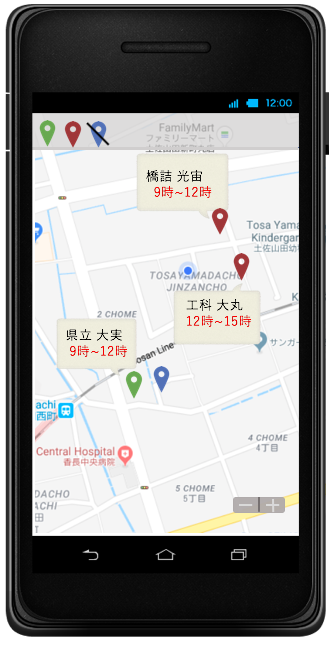
\includegraphics[width=50mm]{map.png}
	\caption{マップ画面}
	\label{fig:map}
 \end{center}

\end{figure}

\newpage

\subsection{利用者側詳細画面}
ここでは配達支援システムの利用者側画面詳細について記します.

\subsubsection{ホーム画面}
図\ref{fig:user_home}は配達支援システムの利用者のホーム画面です.この画面はログイン画面でID,パスワードを入力し,ログインした場合に表示されます.また,既にログインしている場合はアプリ起動時に表示されます.この画面の機能は下記にて説明します.
\begin{enumerate}
	\item 荷物の詳細確認機能\\
	 \ 画面に商品の詳細(商品名,伝票番号,お届け先,お届け日時)を表示しており,荷物を受け取るボタンと日時変更ボタンがあります.荷物を受け取るボタンをタップすると,配達員に網を受け取る通知を送ります.日時変更ボタンをタップすると日時変更画面に遷移します.
	\item 利用者情報ボタン\\
	 \ 利用者のアカウント情報を表示・編集するサイドバーを出すことができます.

	\item 配達済みソートボタン\\
   \ 配達完了状態の荷物の表示・非表示を選択できます.

	\item 受け取り可否別表示ボタン\\
	 \ 「受け取れる」,「受け取れない」,「未選択」の三つを好きに表示・非表示できます.

	\item 検索バー\\
	 \ 入力された文字と一致する荷物を配達時間順(+距離?)に表示します.

\end{enumerate}

\begin{figure}[H]
 \begin{center}
  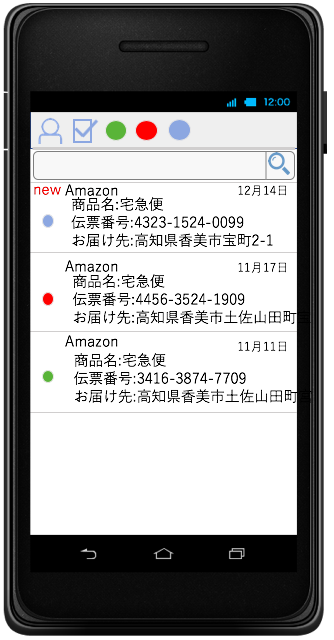
\includegraphics[width=50mm]{user_home.png}
	\caption{ホーム画面}
	\label{fig:user_home}
 \end{center}

\end{figure}
\newpage
\subsubsection{サイドバー画面}
図\ref{fig:user_side}は配達支援システムのサイドバーの画面です.この画面はホーム画面の「利用者情報ボタン」をタップすると表示されます.画面の各欄には利用者の情報(名前,メールアドレス,パスワード,パスワード再入力,電話番号,住所)が表示されており,変更したい部分を書き換えた後に更新ボタンを押すことで利用者情報を変更することができます.また,画面中央上部の「×」ボタンまたはバックボタンをタップするとホーム画面に遷移します.

\begin{figure}[H]
 \begin{center}
  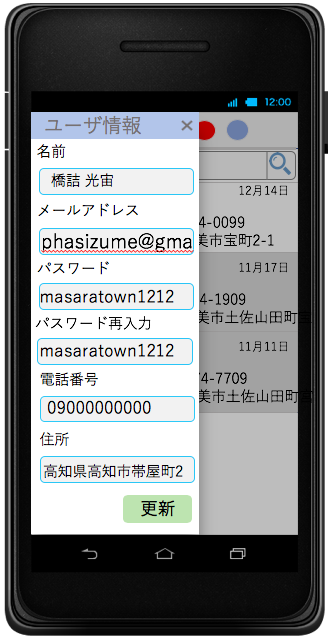
\includegraphics[width=50mm]{user_side.png}
	\caption{サイド画面}
	\label{fig:user_side}
 \end{center}

\end{figure}
\newpage
\subsubsection{詳細画面}
図\ref{fig:user_details}は配達支援システムの利用者詳細画面です.この画面はホーム画面の各荷物欄をタップすると表示され,画面には商品の情報(商品名,伝票番号,お届け先,お届け日時)が表示されます.画面下の「荷物を受け取る」をタップすると配達員に荷物を受け取れると通知され,利用者ホーム画面に遷移します.また,日時変更をタップすると時間変更画面に遷移します.
\begin{figure}[H]
 \begin{center}
  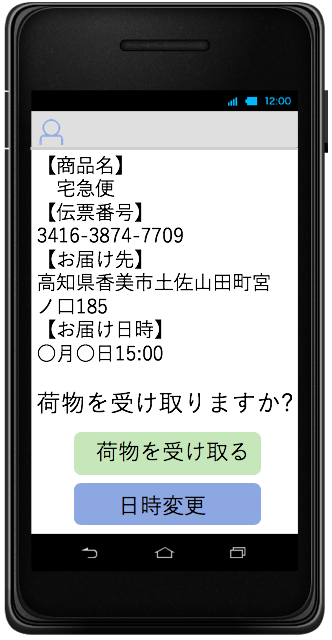
\includegraphics[width=50mm]{user_details.png}
	\caption{詳細画面}
	\label{fig:user_details}
 \end{center}

\end{figure}
\newpage
\subsubsection{日時変更画面}
図\ref{fig:time_change}は配達支援システムの日時変更画面です.この画面は利用者詳細画面の「日時変更」をタップすると表示され,画面には商品の情報(商品名,伝票番号,お届け先,お届け日時)が表示されています.「○月○日15:00お届け予定」の下をタップした後に日時を変更し,「変更確定」をタップすることで配達日時を変更できます.「変更確定」タップ後は利用者ホーム画面に遷移します.

\begin{figure}[H]
 \begin{center}
  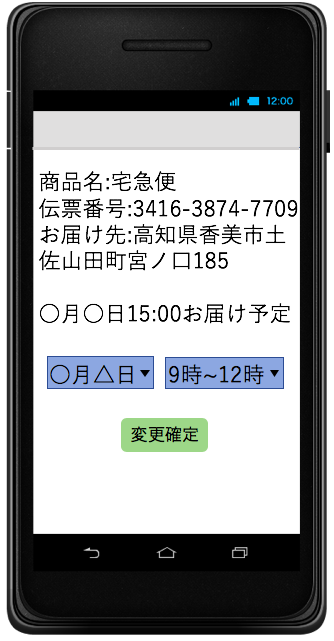
\includegraphics[width=50mm]{time_change.png}
	\caption{時間変更画面}
	\label{fig:time_change}
 \end{center}

\end{figure}
\newpage
\section{システムのハードウェア構成}
本システムのハードウェア構成は表1の通りです.
\begin{table}[H]
\begin{center}
 \caption{ハードウェア構成}
  \begin{tabular}{|c|c|c|}\hline
    項目 & 数量 & 備考\\ \hline \hline
    サーバ & 1台 & AWS\\ \hline
    管理者端末 & 1台 & \\ \hline
  \end{tabular}
\end{center}
\end{table}


\section{ソフトウェア構成}
システム間のやり取りは,Java,MySQLを用いて行います.サーバには,Apache,Tomcat8をインストールして構築しています.

\section{データベース設計}
本システムのデータベースには,5個のデータテーブルを用います.各データテーブルの情報を以下に示します.

\subsubsection{利用者テーブル}
利用者テーブルでは,利用者に関する情報を管理します.このテーブルのデータテーブルを表\ref{userTable}に示します.
\begin{table}[htb]
  \label{userTable}
  \begin{center}
    \begin{tabular}{|c|c|c|c|c|c|} \hline
      属性 & データ型/長 & NULL & Key & 初期値 & その他 \\ \hline \hline
      user\verb|_|id & int(10) unsigned & NO & PRIMARY & NULL & \\ \hline
      name & varchar(64) & NO &   & NULL & \\ \hline
      address & varchar(128) & NO &   & NULL & \\ \hline
      tel & int(11) & NO &   & NULL & \\ \hline
      mail & varchar(64) & NO &   & NULL & \\ \hline
      passwd & vachar(64) & NO &   & NULL & \\ \hline
    \end{tabular}
  \end{center}
\end{table}

\subsubsection{配達者テーブル}
配達者テーブルでは,配達者に関する情報を管理します.このテーブルのデータテーブルを表\ref{driverTable}に示します.
\begin{table}[htb]
  \label{driverTable}
  \begin{center}
    \begin{tabular}{|c|c|c|c|c|c|} \hline
      属性 & データ型/長 & NULL & Key & 初期値 & その他 \\ \hline \hline
      driver\verb|_|id & int(10) unsigned & NO & PRIMARY & NULL & \\ \hline
      name & varchar(64) & NO &   & NULL & \\ \hline
      mail & varchar(64) & NO &   & NULL & \\ \hline
      store\verb|_|code & varchar(64) & NO &   & NULL & \\ \hline
      account\verb|_|type & int(1) unsigned & NO &   & NULL & \\ \hline
      passwd & vachar(64) & NO &   & NULL & \\ \hline
    \end{tabular}
  \end{center}
\end{table}

\subsubsection{商品テーブル}
商品テーブルでは,商品に関する情報を管理します.このテーブルのデータテーブルを表\ref{goodsTable}に示します.
\begin{table}[htb]
  \label{goodsTable}
  \begin{center}
    \begin{tabular}{|c|c|c|c|c|c|} \hline
      属性 & データ型/長 & NULL & Key & 初期値 & その他 \\ \hline \hline
      slip\verb|_|number & int(12) & NO & PRIMARY  & NULL & \\ \hline
      name & varchar(64) & NO &   & NULL & \\ \hline
      address & varchar(128) & NO &   & NULL & \\ \hline
      date & int(10) & NO &   & NULL & \\ \hline
    \end{tabular}
  \end{center}
\end{table}

\subsubsection{管理者テーブル}
管理者テーブルでは,管理者に関する情報を管理します.このテーブルのデータテーブルを表\ref{managerTable}に示します.
\begin{table}[htb]
  \label{managerTable}
  \begin{center}
    \begin{tabular}{|c|c|c|c|c|c|} \hline
      属性 & データ型/長 & NULL & Key & 初期値 & その他 \\ \hline \hline
      manager\verb|_|id & int(1) unsigned & NO & PRIMARY & NULL & \\ \hline
      name & varchar(64) & NO &   & NULL & \\ \hline
      store\verb|_|code & varchar(64) & NO &   & NULL & \\ \hline
      account\verb|_|type & int(1) unsigned & NO &   & NULL & \\ \hline
      passwd & vachar(64) & NO &   & NULL & \\ \hline
    \end{tabular}
  \end{center}
\end{table}

\subsubsection{認証テーブル}
認証テーブルでは,認証に関する情報を管理します.このテーブルのデータテーブルを表\ref{authTable}に示します.
\begin{table}[htb]
  \label{authTable}
  \begin{center}
    \begin{tabular}{|c|c|c|c|c|c|} \hline
      属性 & データ型/長 & NULL & Key & 初期値 & その他 \\ \hline \hline
      user\verb|_|id & int(10) unsigned & NO & FOREIGN & NULL & \\ \hline
      login\verb|_|id & varchar(64) & NO & FOREIGN  & NULL & \\ \hline
      passwd & varchar(64) & NO &   & NULL & \\ \hline
      solt & varchar(64) & NO &  & NULL & \\ \hline
    \end{tabular}
  \end{center}
\end{table}

\section{ネットワーク構成}
本システム全体のネットワーク構成を以下の図\ref{fig:i_f}に示します.

\begin{figure}[H]
 \begin{center}
  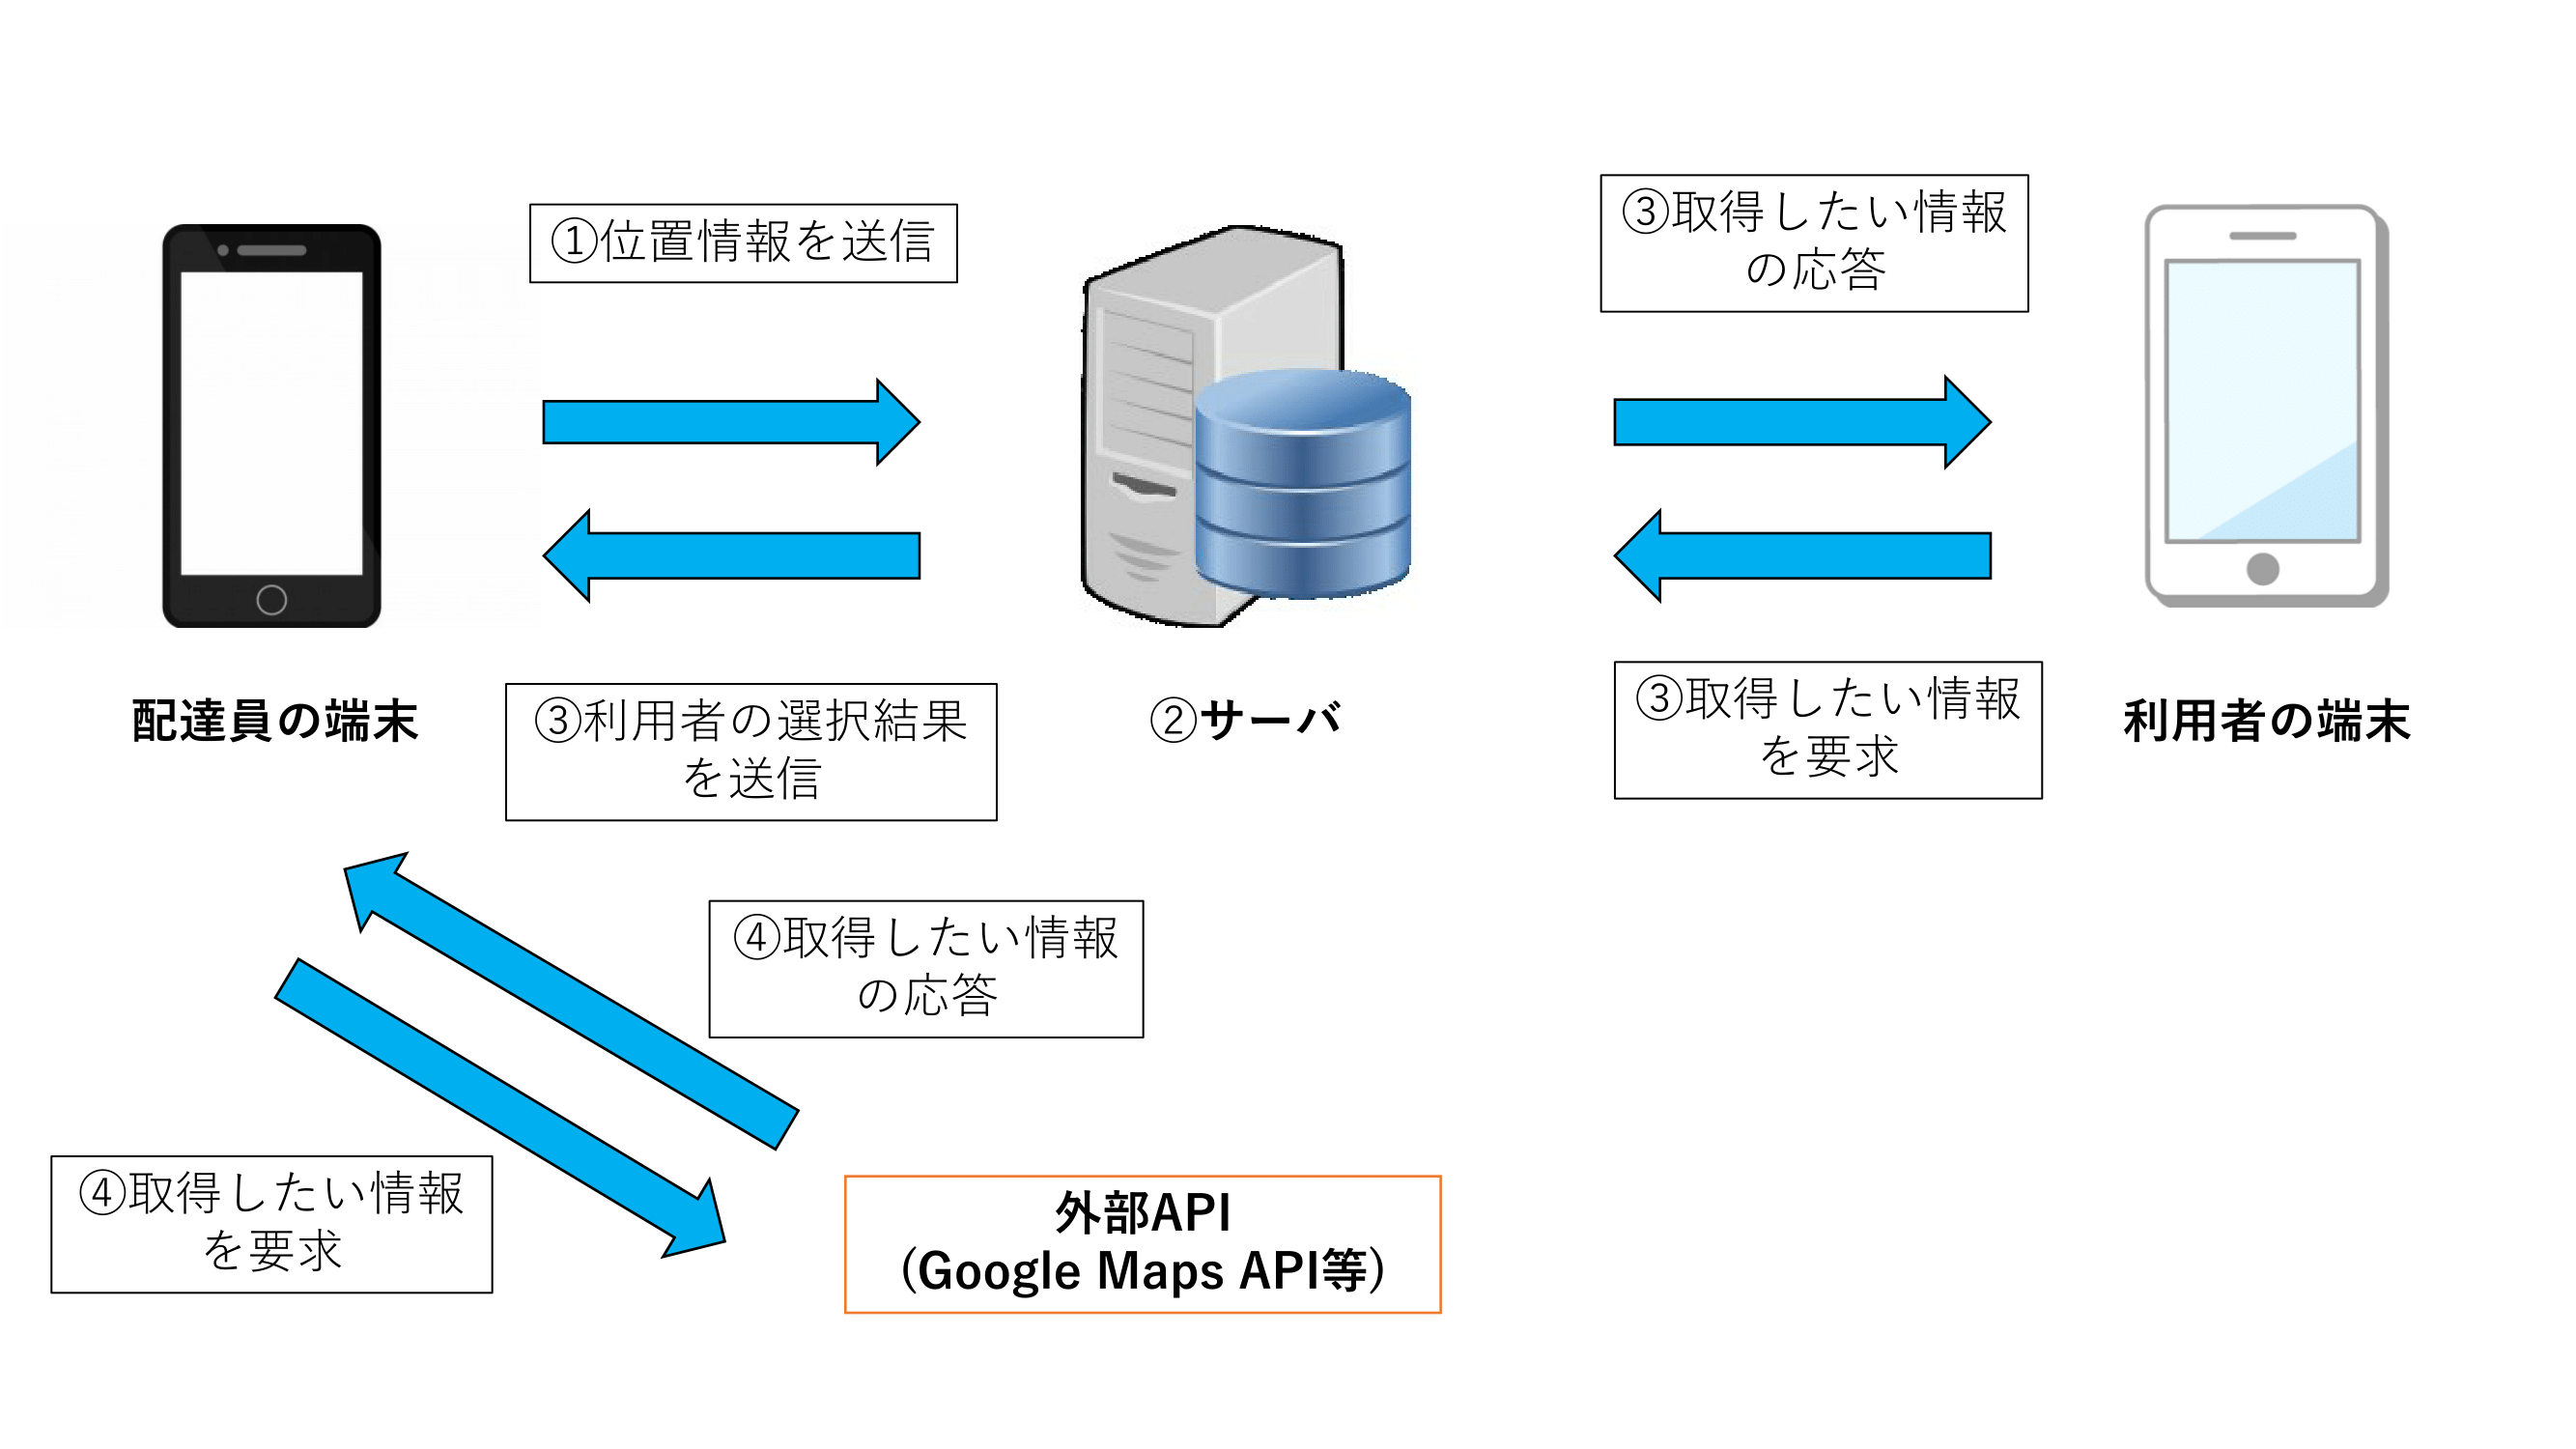
\includegraphics[width=140mm]{information_flow.png}
	\caption{ネットワーク構成}
	\label{fig:i_f}
 \end{center}

\end{figure}


\section{ネットワーク接続形態}
本システムでは利用者端末,管理者端末は TCP/IP を用いてサーバと通信を行います.




\begin{thebibliography}{9}

\bibitem{ref1}
国土交通省,
\newblock ``宅配便の再配達削減に向けて'',\\
\newblock \url{http://www.mlit.go.jp/seisakutokatsu/freight/re_delivery_reduce.html}, \\
2018/10/11
\bibitem{ref2}
エン・ジャパン株式会社,
\newblock ``ヤマト運輸株式会社 中部支社の配達員 ★平均月収35万円。無理なく年収400万円が見込めます。'',\\
\newblock \url{https://employment.en-japan.com/desc_770664/}, \\
2018/10/11
\end{thebibliography}

\end{document}
